%
%-------    Preprint for peer-review
\documentclass[superbib,unsortedaddress,preprint,byrevtex,aps,noshowpacs,titlepage]{revtex4}
%
%
\usepackage{amsmath}
\usepackage{graphicx}
\usepackage{amssymb}
\usepackage{dcolumn}

%%%%%%%%%% ADDONS THAT NEED TO BE COMMENTED OUT IN THE FINAL VERSION
\usepackage[pdftex,                 %
            colorlinks,             %
            linktocpage,            %
            breaklinks,             %
            bookmarks=true,         %
            bookmarksnumbered=true, %
            citecolor=blue]{hyperref}
\usepackage{breakurl}
\usepackage[color=red!40!]{todonotes}
\usepackage[utf8]{inputenc}
\usepackage[T1]{fontenc}
\setlength\oddsidemargin{-0.5in}
\setlength{\marginparwidth}{80pt}
\def\mytodo#1{$\clubsuit$\todo[noline]{$\clubsuit$\,\,\footnotesize #1}}

\hypersetup{
  pdfauthor = {Domingos Rodrigues},
  pdftitle = {Paper que ja devia ter sido submetido faz tempo},
  pdfsubject = {algoritmos geneticos em liberacao controlada de drogas},
  pdfkeywords = {algoritmo genetico, liberacao controlada de drogas},
  pdfcreator = {LaTeX with hyperref package},
  pdfproducer = {pdflatex}
}

\pdfadjustspacing=1

%%%%%%%%%% ADDONS THAT NEED TO BE COMMENTED OUT IN THE FINAL VERSION


% Endfloat class option:
%  It is used to put off all floats (including figures and tables) to 
%  wherever with the command \printfigures. 
%  endfloat*, by default, will put figures after the end of text. 
%  \listoffigures is used to generate a list of figure captions. 
%  \listoftables does the same thing for tables. 
%  RevTeX has a bug concerning listoffigures, which might be worked around 
%  by inserting in the preamble the following redefinitions of the dot separation 
%  distance:

\makeatletter
\def\@dotsep{4.5}
\makeatother

\def\vchi{\roarrow{\chi}}
\def\vchiref{\roarrow{\chi}_\text{ref}}
\def\Qref{Q_\text{ref}}
\def\calF{\mathcal{F}}
\def\Co{C_0}
\def\Cs{C_\text{s}}

\bibliographystyle{apsrmp}
%---------------------------------------------------------------------------------
%
%
%                                      DOCUMENT
%
%
%---------------------------------------------------------------------------------

\begin{document}

\preprint{}


\title{An Adaptive Fuzzy-Genetic Algorithm for estimating matrix
  physicochemical properties to achieve desired drug release 
  profiles.}

\author{Domingos D. C.\ Rodrigues}
\affiliation{%
  Centro Nacional de Processamento de Alto Desempenho, %
  Laborat\'orio de Computa\c{c}\~ao Cient\'{i}fica-ICEx, %
  Universidade Federal de Minas Gerais, Pampulha (31.270-901) Belo %
  Horizonte, MG-Brazil} 

\author{Cláudio César F. Ale Almeida }
\email{ccesar@dcc.ufmg.br}
\affiliation{%
  Departamento de Ciência da Computação-ICEx, Universidade Federal de Minas Gerais, %
  Pampulha (31.270-901) Belo Horizonte, MG-Brazil
}

\author{Jadson C.\ Belchior}
\email{jadson@ufmg.br}

\affiliation{%
  Departamento de Qu\'{i}mica-ICEx, Universidade Federal de Minas Gerais, %
  Pampulha (31.270-901) Belo Horizonte, MG-Brazil
}

\author{José Lopes de Siqueira Neto}
\email{jose@dcc.ufmg.br}

\affiliation{%
  Departamento de Ciência da Computação-ICEx, Universidade Federal de Minas Gerais, %
  Pampulha (31.270-901) Belo Horizonte, MG-Brazil
}

% ---------------------------------------------------------------------

\begin{abstract}

  %\todo[inline]{ULTIMA COISA A SER FEITA DEPOIS DE TERMOS UM CORPO DE ARTIGO ...}
  \vskip\baselineskip
	
	An alternative methodology based on genetic algorithm is proposed to be a complementary tool to other conventional methods to study controlled drug release. Two systems are used to test the approach; namely, hydrocortisone in a biodegradable matrix and rhodium (II) butyrate complexes in a bioceramic matrix. Two well-established mathematical models are used to simulate different release profiles
as a function of fundamental properties; namely, diffusion coefficient (D), saturation
solubility (Cs), drug loading (A), and the height of the device (h). The models were tested,
and the results show that a wide range of values for these fundamental properties can be predicted to achieve the desired drug release. The genetic algorithm results obtained can be considered to quantitatively predict ideal experimental conditions. Overall, the proposed methodology was shown to be efficient for ideal experiments, with a relative average error of <1\% in both tests. This approach can be useful for the experimental analysis to simulate and design efficient controlled drug release systems.
  
\end{abstract}

\pacs{xx.xx.xx, xx.xx.-x, xx.xx.-x}

\date{\today}

% ---------------------------------------------------------------------

\maketitle

\section{\label{sec:intro} Introduction}

Over recent years there has been a growing interest in drug delivery
studies from solid pharmaceutical dosage forms.
Drug delivery systems (DDS hereinafter) must be developed taking into
account the economical aspects involved in the industrial mass
production, that is to say that DDS must be manufactured at low cost
without compromising the therapeutic goal of the drug. 
This has prompted the pharmaceutical industry to search for new cheap raw
materials for the manufacture of delivery systems and for the formulation
of new encapsulation techniques (\cite{Siepmann2001b} and references
therein).
It is therefore important to be able to quantify the dependence of the transport
mechanisms involved in the release of any drug from the physicochemical properties
of the carrier material.
In general the therapeutic treatments consist in delivering the drug to some specific
region or organ of the body which therefore requires that the medication must be released
in a controlled and sustained form to keep its concentration in the body at accepted levels.
Due to ease of production and low cost associated, the usual procedure is to disperse 
some drug in a hydrophobic (e.g.%
%%%%%
%%\mytodo{exemplos}) %
%%%%%
or hydrophilic (e.g.\, hydroxypropyl methylcellulose-HPMC) biomaterial so that a controlled release of the 
drug into the biological medium can be attained. 
In the pharmaceutical literature this combination of drug and excipient agent is commonly
referred as matrix.
Overall the release of any drug from some matrix (consisting of bioceramics or biodegradable polymers) 
involves both the physical phenomena of dissolution or erosion and diffusion. 
Once the tablet carrying the drug in suspension enters in contact with water or the physiological fluid,
 the latter diffuses into the tablet (imbibition) increasing its 
volume (swelling) and promoting the drug dissolution. 
The dissolved drug will then diffuse out of the device due to steep concentration gradients. 
For water insoluble polymers, the diffusional mass transfer is preceded by cleavage of the 
polymer chains that constitute the matrix (erosion). 

Several phenomenological models have been proposed with various degrees of
sophistication to describe such processes in simple and compact mathematical forms 
(for a comprehensive review see~\cite{Costa2001}), but full treatment
of the involved transport mechanisms often need to be done numerically.
When no matrix erosion or swelling occurs (or they are instantaneous) and drug molecules do not
interact, the release is basically controlled by the mechanism of Fickian diffusion which is a well
 understood process with a very precise mathematical formulation for any geometry of the device 
and deeply rooted in physical first principles (~\cite{Crank1975}). 
Even so, simple analytical solutions are only obtained when one imposes strict assumptions, as 
constant drug diffusivity, perfect sink conditions, fixed boundaries
and an infinite external medium.
When dissolution or erosion becomes relevant, the resulting mathematical equations
can get somewhat cumbersome as the drug diffusion in a substrate can depend on various 
parameters, such as the matrix composition, matrix geometry, volume expansion 
(swelling), erosion, polymer dissolution, initial drug loading and drug saturation solubility 
in the matrix~\cite{Siepmann2001,Siepmann2001b}. 
Therefore depending on the degree of simplification of the kinetics behind drug release, one
can get an explicit or implicit analytical relation between the independent (mass-fraction 
of drug release and time) and dependent (physicochemical properties of the matrix) variables 
of the problem.

From the technological point of view, explicit analytical formulas as simple as possible are mostly
desired in order to simulate and access the economical viability of alternative paths of the 
manufacturing of DDS in a rapid and efficient manner, as well as for routine quality control processes. 
Several statistical methods have been proposed to test the similarity between dissolution profiles
of test and reference batches as well as to decide the best model to study the drug dissolution (
we refer the reader to the review of~\textcite{Costa2001}).
Given the elevated number of variables involved, one does in practice several cuts in the
parameter space and performs a nonlinear regression analysis to fit the experimental
data to some chosen model~\cite{Fu1976}.
Quite recently a complementary approach to these conventional methods based on artificial neural 
networks (AAN) has been used (see review of ~\textcite{Sun2003} and references therein). 
This approach has proved to be useful in predicting ideal experimental parameters 
for providing a controlled drug release. 
It uses the whole experimental data training set and correlates it with the input parameters of 
the chosen formulation by optimizing the weights and biases of the ANN through some minimization 
technique. 
There is no need to have {\it a priori} functional relationship between the dependent and
independent variables although in practice one uses some accepted model to simulate a great
number of experiments to increase the training set. 
After the training stage, one can quickly predict new formulation input parameters (geometry
and physicochemical properties of the matrix) for any dissolution profile of any new submitted 
experimental batch (assuming the experimental conditions have been maintained as those of the 
training set). The use of ANNs is nevertheless limited, as they cannot provide any information
at all about the underlying mechanisms of drug dissolution and diffusion.
It was in this context that ~\textcite{Reis2004} showed the usefulness of the ANN methodology
by applying it to real experimental systems, namely the hydrocortisone in a biodegradable 
matrix and rhodium (II) butyrate complexes in bioceramic matrices.
The training set consisted of hydrocortisone experimental data compiled by ~\textcite{Fu1976} plus 
artificial data created using the Higuchi equation with variation of the physicochemical parameters 
of~\textcite{Fu1976} within specified bounds.
They have shown that submitting a new unknown experimental data set to the neural network 
the algorithm was able to recover the input parameters of the formulation (drug solubility, 
initial drug loading and radius and thickness of tablet) for short and long time period releases. 
They have nevertheless noted that either ANNs or conventional methods, as nonlinear regression 
analysis, only provide a single possible set of parameters for some experimental release 
profile as this is essentially a multivariate problem.

Therefore it is desirable from the experimental point of view to have a whole spectrum 
(not necessarily complete) of physicochemical parameter values for some matrix that once combined 
reproduce its fiducial drug release fractions at pre-specified intervals of time.
With this background data new unforeseen experimental paths may be explored in order to get new matrix
compositions and geometries that may be economically more viable yet 

In the following sections, we show how the above multivalued parameter problem can
be casted into a numerical optimization problem generally known as multimodal function 
minimization.
We subsequently describe the methodology used in this work, which is based on a genetic algorithm.
We use the Higuchi semi-empirical model (Section~\ref{sec:higuchi}) in
our benchmarks due to its analytical simplicity and widespread use.
Nevertheless the proposed algorithm can be easily applied to any other more sophisticated
drug release model, but with a possible higher cost in computational resources. 

\section{Methodology}

\subsection{Drug release mathematical formulation}
\label{sec:higuchi}

Following our previous work~\cite{Reis2004} we use the model proposed by~\textcite{Higuchi1961} 
for our fiducial controlled release profile of HPMC tablets.
This theoretical model was originally proposed with the intent of studying the release of drug 
molecules from creams and ointments, but since then has found widespread use in controlled delivery 
systems based on HPMC~\cite{Costa2001,Siepmann2001}.
~\textcite{Higuchi1961} assumed a one-dimensional system (slab model) under pseudo-steady 
conditions which generally cannot be applied to real controlled released systems.
As illustrated in Fig.~\ref{fig:sketch} the model assumes that as time evolves three distinct regions 
along the cross section of a thin tablet appear. 
In the pristine region III the drug is assumed to be in solid form, finely divided and in an immobile 
dispersed state within the matrix with some constant initial concentration $\Co$. 
As the tablet enters in contact with some external medium (region I) an intermediate region II starts 
to develop, where the drug is completely dissolved and with concentration below the solubility 
limit $\Cs$. 
As the dissolution front, $x_b$, moves with time the dissolved
drug diffuses through the boundary $x = 0$ to some external reservoir. 
The external reservoir is assumed to be very large and well-mixed so that perfect sink conditions
are maintained at the surface of the carrier ($C(0,t) = 0$).
Given this simplified setting a few additional assumptions underpin the derivation of the Higuchi equation:
the dissolution rate is faster than the drug diffusion rate;
swelling or erosion of the carrier is negligible (dimensions of tablet are kept fixed);
the initial loading is much greater than the drug solubility in the matrix ($R=\Cs/\Co \ll 1$);
and finally the concentration profile is linear inside the depletion zone 
(region II in Fig.~\ref{fig:sketch}).
This pseudo-steady state is a reasonable approximation as long as there is a relatively large excess 
of dispersed solute ($R \le 1$). 
The moving front, $x_b(t)$, will then be located so that the mass of drug which has dissolved and left 
region III is equal to the mass diffused across the boundary $x=0$.
Using the Fick's second law of diffusion at boundary $x=0$~\cite{Crank1975} one can easily derive 
an expression for $x_b$:

\begin{equation}
  \label{eq:moving_bc}
  x_b(t) = \left[\frac{2DRt}{1-R/2}\right]^{\frac{1}{2}}.
\end{equation}

From Eq.~\ref{eq:moving_bc} one can derive the cumulative mass fraction of suspended drug, 
$Q(t)$, that has been released to the external medium:

\begin{equation}
  \label{eq:higuchi}
  Q(t) = \left[\frac{2RD}{L^2}\left(1-\frac{R}{2}\right)\right]^\frac{1}{2} t^{1/2}
\end{equation}

where $Q(t) = M_D(t)/M_\text{tot}$, with $M_D$ and $M_\text{tot}$ being respectively the diffused 
and total drug masses, $D$ is the effective diffusivity of the drug molecules in the matrix substance,
 assumed to be constant, and $L$ is the total thickness of the topical formulation.

Equation (\ref{eq:higuchi}) remains valid as long as $R$ is significantly small. 
Once the parameter $R$ approaches unity, when most of the drug has dissolved, the
pseudo-steady state is no longer valid and subsequent drug diffusion is governed by some 
unsteady-state diffusion solution (see~\cite{Bunge1998}).
The exact solution for the above simplified model with drug in suspension for all concentration
 ratios $R<1$ was found by~\textcite{Paul1976}, who do not assumed a linear drug concentration 
within the dissolved zone.
Although more complicated than the Higuchi solution (Eq.~\ref{eq:higuchi}), their exact solution confirms 
the power-law behaviour with time as long as some drug remains in the solid phase.
\textcite{Bunge1998} made a thoroughly comparison between predictions of the Higuchi approximation and the
exact solution by varying the parameter $R$. 
She found that the Higuchi approximation underpredicts the cumulative mass released by a few ten percent 
when $R$ approaches unity.
A direct consequence of this is that the relative error of the constant of diffusion, $D$, if estimated
from experimental data of the cumulative mass released, may reach about $30\text{\%}$.
The Higuchi approximation also overpredicts the time required for complete dissolution of the drug.
In order to minimize these differences, \textcite{Bunge1998} proposed a simple modification of 
Eq.~\ref{eq:higuchi}:

\begin{equation}
  \label{eq:higuchi_mod}
  Q(t) = \left[\frac{2RD}{L^2}\left(1-\frac{R(\pi-2)}{\pi}\right)\right]^\frac{1}{2} t^{1/2}
\end{equation}

Despite all the above restrictions, the Higuchi approximation still provides a reasonable 
description of the mass released from suspended drugs with $0 < R < 1$ (see Fig.5 from~\textcite{Bunge1998})
and thus we will use Eq.~\ref{eq:higuchi} in the forthcoming sections.
We should refer in passing that the proportionality between the fractional amount of drug released
and the square-root of time can be also derived from different physical grounds, namely from the
diffusion of the drug not initially present in solid form, that is with $\Co < \Cs$, for thin films 
under perfect sink conditions and constant diffusivity~\cite{Crank1975}.  

We remind the reader that if one assumes a more complicated device geometry
or a more comprehensive mechanistic theory, more complex non-analytical descriptions will be obtained for 
the drug release rates (for the slab geometry with more elaborated release kinetics see for 
example \cite{Frenning2003,Kalia2001a} and references therein; for cylindrical geometries see 
the comprehensive reviews in ~\cite{Siepmann2000,Siepmann2001,Siepmann2002}). 
However if one intends to have a first hand knowledge of a new topical formulation, then the Higuchi 
power-law approximation will suffice and will have the extra advantage of low computational cost.

\subsection{Genetic Algorithmic approach}
\label{meth:ga}

According to Higuchi's power-law (Eq.~\ref{eq:higuchi}) the constant of proportionality incorporates 
all the structural and geometric characteristics of the carrier device and so a multitude of physically acceptable
combinations of the parameters $\Co$, $\Cs$, $D$ and $L$ can give equivalent mass release profiles. 
We propose in this section a methodology based on genetic algorithm fundamental concepts for finding all 
relevant sets of parameters $\vchi = \{\Co,\Cs, D, L\}$ that give the same mass release profile $Q$ as some 
chosen reference profile $\Qref$.
In the present work we adopt an artificial reference profile, $\Qref$, the same as that introduced
by ~\cite{Reis2004} to validate their neural network model of controlled drug release 
(see Table~\ref{tab:ranges}).   
Let us then define the following functional:

\begin{equation}
  \label{eq:fitness}
  \calF(Q(\vchi)) = \log \left| \frac{Q(\vchi; t)}{Q(\vchiref; t)} - 1 \right|,
\end{equation}

where the function $Q$ is given by Eq.~\ref{eq:higuchi} and $\vchiref$ is the vector of parameters for 
our reference profile.
Recall that $\calF$ is independent of the time variable, $t$, because $Q$ is a power-law, but if $Q$ has
a different functional form, one or more instants of time (e.g. the dissolution time) needs to be added
to the parameter space $\vchi$.
%due to the power-law behaviour of Eq.~\ref{eq:higuchi}, but for a
%different functional form one or more instants of time (for example the dissolution time) need to be added to the 
%parameter space $\vchi$.
From now on we will drop the variables from the definition of $Q$ to avoid cluttering of the equations.
One can easily see that the function $\calF$ diverges whenever the trial function $Q$ tends to $\Qref$. 
Moreover as expected, there is more than one solution $Q$ for which $\calF$ diverges, as can be seen 
by inspection of Figures (\ref{fig:higuchi}) and (\ref{fig:higuchi_zoom}).
There we plot the projections of the $4$-dimensional landscape of the function $\calF$ on all planes defined by 
the pairing of the variables $\Co$, $\Cs$, $D$ and $L$.
Distinctive features are revealed in those figures, namely an aligned set of disjoint regions 
with negative elliptical contours present in all projections of $\calF$.
% Truly these minima regions result from the numerical resolution of the hyper-surface, 
% since formally $\calF$ tends to $-\infty$ at these critical points.
As these regions are zoomed up (Fig.~\ref{fig:higuchi_zoom}) the elliptical contours merge to form
long ridges that in turn reveal another set of elliptical contoured regions of decreasing value
of $\calF$ in a self-similar fashion.
Given this, one easily realizes that the set of minima simply correspond to the set of mass release 
functions, $Q= K(\vchi) t^{1/2}$, for which $|K-K_\text{ref}|<\epsilon$ with $\epsilon$ being very small. 
That is, one can cast the combinatorial problem of finding all possible combinations among the parameters 
$\{\Co, \Cs, D, L\}$, that give almost the same value of $K_\text{ref}$, to the optimization task of locating 
all minima in the $4$-dimensional hyper-surface of $\calF$ as defined in Eq.~\ref{eq:fitness}.
To solve this optimization problem we make use of a genetic algorithm technique (hereinafter GA).

Standard genetic algorithms are known to be a particularly good approach for optimization problems that require
finding either a unique global solution
%, for example some global minimum, %
%%%%%
%\mytodo{Talvez aqui podem vir as refer\^encias de trabalhos de clusters at\^omicos} %
%%%%
or more than one solution like the work discussed in here (see for example~\cite{Goldberg1989,Kao2008}).

Unlike local traditional optimizers, like the first-order (steepest descent, conjugate gradient) and 
second-order (quasi-Newton) methods, GAs are stochastic search methods not strongly influenced by the 
initial trial solution. 
This is because the genetic algorithm paradigm consists in evolving a group of candidate solutions 
(population) throughout a number of steps, where at each new step (generation) a new group of solutions is created
 from the previous one by a set of transformations. 
These transformations, inspired by the laws of natural selection, comprise the basic
 operations of recombination of the information encoded in some probabilistically selected pairs of solutions among
the population accompanied by some random alteration of the encoding in their offspring. 
The fittest members of the population of solutions according to some figure of merit, the fitness function, will pass 
onto the next generations preserving most of their optimal information~\cite{Goldberg1989}.
All this enables the GA method to explore new points in the search space and proves quite effective in locating
the global minimum of some complicated functions which is masked by a plethora of local minima %
%%%%
%% \mytodo{Refer\^encia a clusters at\^omicos?} %
%%%%
and could not possibly be found by the more traditional search procedures (unless of course some finely 
tuned initial trial solution is provided in the neighborhood of the global minimum, but that is 
completely unknown {\it a priori}).
The choice of GA parameters, such as the selection method for crossover and mutation operations and their 
associated frequency of occurrence, determines the balance of exploration of search space and the exploitation of
information contained in the population. 
It is the adequacy of this balance that leads to the successful application of a GA.
Instead we try to ameliorate this situation by introducing new genetic operators.
Three new genetic operators are introduced: the predator operator, a new niche %
%%%%%
% \mytodo{niche ou habitat ?} %
%%%%5
operator that we call the habitat operator and finally the immigration operator.
They are all designed in order to preserve "speciation", that is, to locate new distinct clusters (species) of
solutions and to preserve as best as possible the neighborhoods around local minima already found 
by the algorithm.

We proceed by describing the main features of the new proposed genetic algorithm (GA).
The search run is started with a population of $100$ trial profiles each of which represented by
a key-value, where the value is a $4$-dimensional vector $\vchi$ of key-value: 

I = F-$\{\Co-Cobin,\Cs-Csbin, D-Dbin, L-Lbin\}$

where:

\begin{itemize}
	\item \textbf{F} is the individual fitness
	\item \textbf{Co} is the decimal value of the parameter Co (phenotype)
	\item \textbf{Cobin} is a customized binary representation of the parameter Co (chromosome)
	\item \textbf{Cs} is the decimal value of the parameter Cs (phenotype)
	\item \textbf{Csbin} is a customized binary representation of the parameter Cs (chromosome)
	\item \textbf{D} is the decimal value of the parameter D (phenotype)
	\item \textbf{Dbin} is a customized binary representation of the parameter D (chromosome)
	\item \textbf{L} is the decimal value of the parameter L (phenotype)
	\item \textbf{Lbin} is a customized binary representation of the parameter L (chromosome)
\end{itemize}

%As in the standard GA, the real components of the vectors are encoded into binary strings and 
%these are concatenated to form a long string to represent the vector $\vchi$, called in the GA 
%jargon by chromosome.
The search space of each of the vector components of $\vchi$ is bounded by the intervals listed 
in Table~\ref{tab:ranges}. 
We require that multiple solutions $\vchi$ found by the GA must be 
distinguished experimentally so we must restrict the arithmetic precisions of their components 
accordingly. 
Given the ranges listed in Table~\ref{tab:ranges}, we encode each of the components $\Co$, $\Cs$, $D$, $L$ with $32$ bit long strings respectively.
%% We require for each vector component, $\Co$, $\Cs$, $D$, $L$, a precision of $??$ digits after the decimal point
%% restrict their values within the ranges that are listed in Table~\ref{tab:ranges}.
This means that a total of $128$ bits are necessary to represent the whole genotype - all the chromosomes.
The ranges in Table~\ref{tab:ranges} define an envelop around the reference Higuchi profile 
$Q(t;\vchiref)$ and we always start the GA with a population of random profiles constrained to
this region.

As the GA is designed to give multiple profile solutions one needs to find only the most 
representative and eliminate very similar profiles. 
We do that by grouping several solutions into sets of clusters (classes), each of which contains 
profiles that have very similar parameters according to the classification system%
%%%%%
%%\mytodo{Falta especificar a convers\~ao do string bin\'ario para o par\^ametro $\in [0,1]$}
%%%%%
 that will be described later.

The GA starts by generating a random population of 

% \todo[inline]{%
%   Aqui devemos introduzir os novos operadores gen\'eticos \`a medida que descrevemos os passos
%   do algoritmo gen\'etico.
%   Para cada operador devemos introduzir as fun\c{c}\~oes de pertin\^encia ({\it membership functions}) e 
%   seus par\^ametros. No caso de fun\c{c}\~oes com constantes devemos dizer porque foram usados esses valores
%   para as constantes, isto \'e, como foram calibradas essas fun\c{c}\~oes. Talvez, devessemos explicar
%   no come\c{c}o desta sec\c{c}\~ao a liga\c{c}\~ao que fazemos entre a l\'ogica {\it fuzzy} e os operadores 
%   gen\'eticos.
%   Outra coisa que voc\^es deveriam verificar \'e que as sigm\'oides s\~ao abertas para a direita apenas 
%   para alguns intervalos de $M$ e $D$, sendo $M$ e $D$ respectivamente a m\'edia e a dispers\~ao dos 
%   valores de {\it fitness} para a popula\c{c}\~ao. Para outros intervalos, a sigm\'oide \'e aberta para a
%   esquerda. Importa?
%   N\~ao ficou claro para mim a fun\c{c}\~ao respeitante ao operador {\it crossover}. Trata-se de um produto 
%   alg\'ebrico de duas sigm\'oides? Como \'e efetuado o {\it crossover}? Em quantas partes \'e dividido o 
%   cromossoma representante da solu\c{c}\~ao para fazer a recombina\c{c}\~ao?
%   Tamb\'em \'e necess\'ario explicar melhor os crit\'erios de converg\^encia do algoritmo. O que significa 
%   Erro$_\text{limite}$ e Desvio$_\text{Limite}$? Como est\~ao definidos?
% }

\missingfigure{Falta colocar o {\it flowchart} do algoritmo gen\'etico}

\section{Results and discussion}

%\missingfigure{Falta colocar os gr\'aficos que d\~ao o {\it fitness} e o n\'umero de solu\c{c}\~oes em fun\c{c}\~ao
%  da gera\c{c}\~ao.
%}

% \todo[inline]{Devemos discutir os resultados da tabela~\ref{tab:results} n\~ao s\'o 
%   apresent\'a-la. Por exemplo os tempos de dissolu\c{c}\~ao completa da droga na matriz
%   v\~ao ser diferentes para cada conjunto de par\^ametros. Talvez seja necess\'ario
%   apresentar tamb\'em alguns valores experimentais da literatura para comparar com os
%   valores obtidos. Certamente alguns conjuntos de par\^ametros simulados n\~ao devem ser 
%   realiz\'aveis experimentalmente.
% }

\section{Concluding remarks}

We have argued in this work the technological importance of being able to estimate 
sets of possible combinations of physicochemical properties of a drug-matrix system 
that can achieve the same desired drug controlled release profile.
This ability allows a rapid and efficient assessment of the economical viability
of the different paths of tablet manufacturing that might be proposed according to the
therapeutic goal of the drug, the physiological medium where the drug is supposed to 
be most effective or the timing of some fixed drug fraction.
Evidently not all parameter combinations might be experimentally possible, but that 
provides precisely the argument in favour of being able to generate large batches 
of parameters at once so that one can quickly inspect and select the most feasible 
combinations.
The adaptive genetic algorithm described in here proved to be an efficient pratical tool 
in achieving the above goals.
%
% MELHORAR ISTO AQUI!
%
% Despite the test case being formally quite simple, namely the Higuchi power-law 
% where all physicochemical parameters are combined into just a single factor, it
% reveals itself difficult in practice to find systematically all desired combinations
% without the aid of some intelligent system.
The release profile we used as a test case for our algorithm even being formally quite
simple, all physicochemical parameters combined into just a single factor, it clearly 
showed how difficult is in practice to find systematically all targeted combinations
of the physicochemical parameters of the drug-matrix composition without the aid of 
some computational intelligent system.  
One should remind the reader that our genetic algorithm is also a generic
search tool in the sense that it does not require that the controlled release model 
must be expressed analytically.
All that our GA requires from any drug release model is the evaluation of the fitness function
 (~\ref{eq:fitness}), either by direct evaluation of some analytical expression or by the 
numerical resolution of a set of coupled differential equations (e.g.~\cite{Siepmann2000,Siepmann2002}).
% at the expense of higher computational demands and slower convergence.
In either situation one may have to tune the action of the genetic operators if
the dimensionality of the search space increases as well as the complexity of its 
topology depending on the particular release model under study.

\cite{}

% Finally, if one is not only interested in obtaining sets of parameters that originate
% release profiles infinitely similar to the desire one, but also profiles which lie 
% within some envelop all we need is to relax the convergence criterion.

% \todo[inline]{O que eu quero dizer na \'ultima frase \'e aumentar o desvio m\'edio requerido 
%   das curvas em rela\c{c}\~ao \`a curva padr\~ao que \'e requerido para a converg\^encia do GA
%   (isto \'e, aumentar o valor limite de $\epsilon$ da tabela ~\ref{tab:results})
% }

\section*{Acknowledgments}

% =============================================================================
%
% When manuscript is ready for submission replace the
% line below with the file produced by the python script process_bib.py
%
\bibliography{drug_release}
 
% \begin{thebibliography}{23}
% \end{thebibliography} 

\clearpage

\listoffigures

\clearpage

\listoftables

\clearpage

% =============================================================================

%
%  ----- only figure captions. Figures by themselves are annexed
%
% In order to produce a list of figure captions with only the first sentence or 
% a few keywords, write \caption[the key words to be printed in the list]{full caption}.
%
\begin{figure}
  \centering
  % \includegraphics[type=eps,ext=.eps,read=.eps,width=0.75\textwidth]{figures/sketch}
  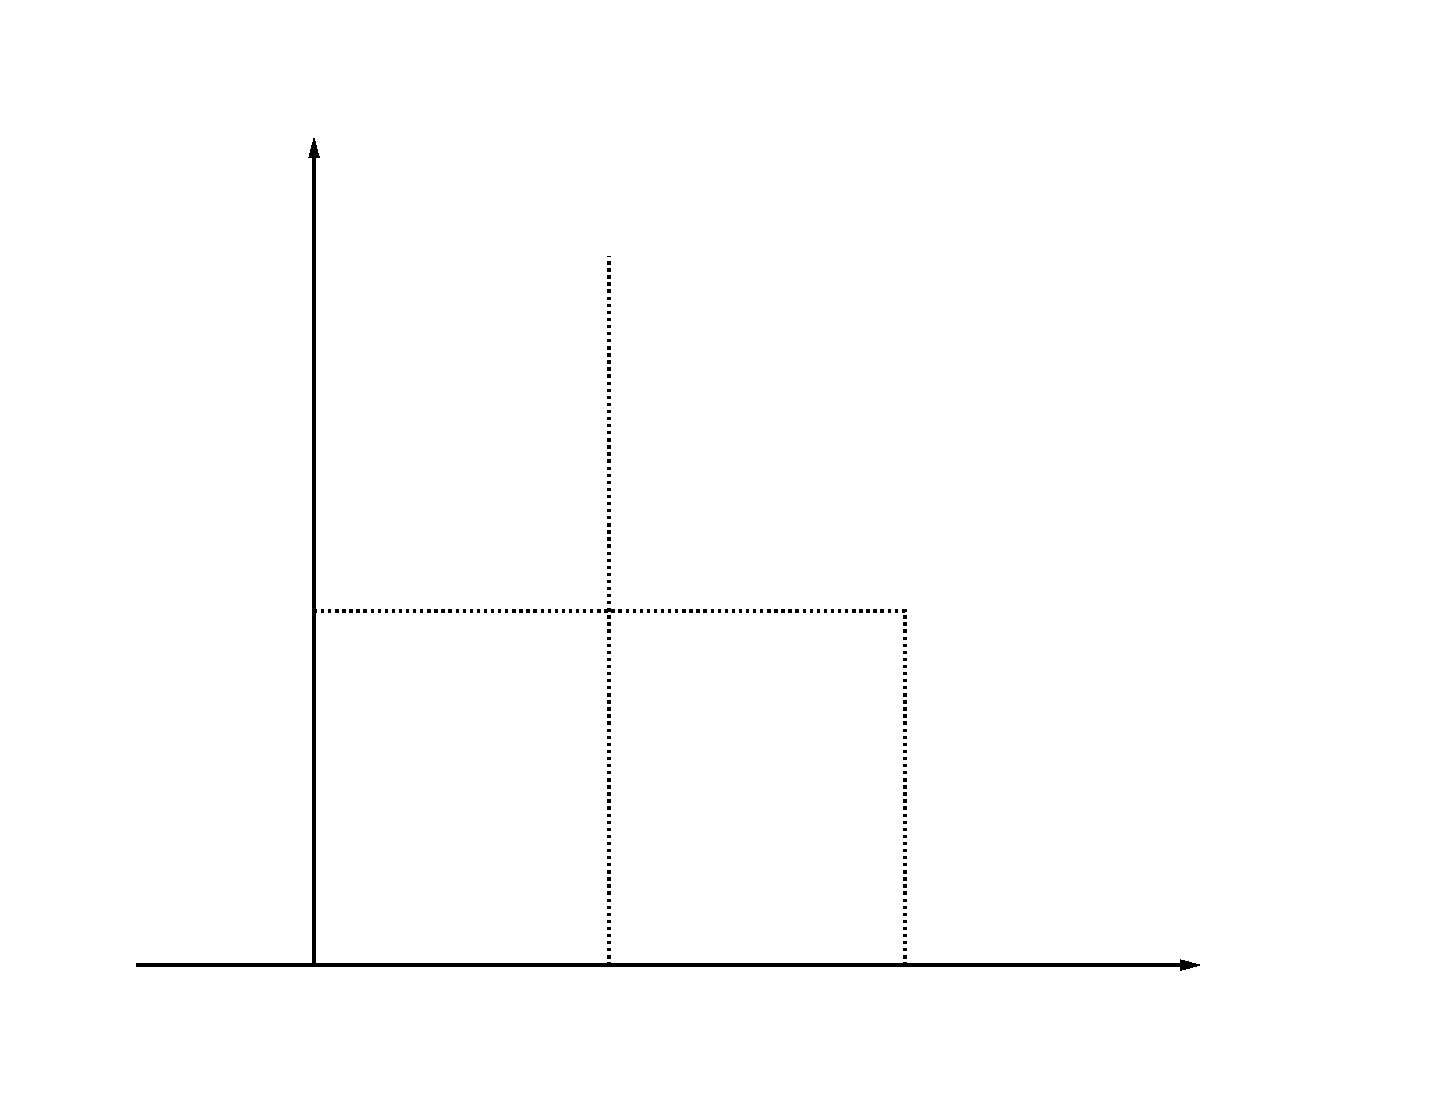
\includegraphics[width=0.75\textwidth]{figures/higuchi_sketch.eps}
  \caption{Diagram showing the drug concentration profile at time $t$ in some planar 
    thin matrix of half-thickness $L/2$ (thick line). 
    Diffusion proceeds along the horizontal axis from region $II$, where the drug is
    completely dissolved, to an external sink (region $I$). Meanwhile the boundary 
    between regions $II$ and $III$, $x_b(t)$, moves along the positive direction of the 
    $x$ axis as the suspended drug in region $III$ dissolves with time.} 
  \label{fig:sketch}
\end{figure}
\clearpage

\begin{figure}
  \centering
  %\includegraphics[type=eps,ext=.eps,read=.eps,width=0.75\textwidth]{figures/higuchi}
  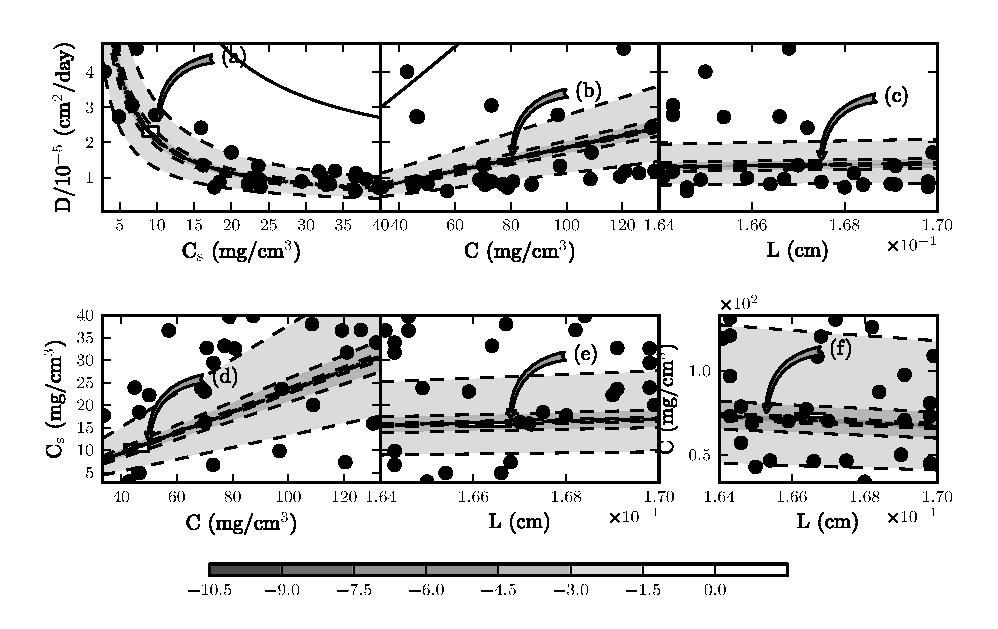
\includegraphics[width=0.75\textwidth]{figures/higuchi_proj.eps}
  \caption{Filled contour plots representing the projections of the four-dimensional
    function $\calF$ (Eq. ~\ref{eq:fitness}) onto the planes (a) $D$-$\Cs$, (b) $D$-$\Co$, 
    (c) $D$-$L$, (d) $\Cs$-$C$, (e) $\Cs$-$L$ and (f) $C$-$L$. Dashed lines refer to 
    contours with negative values. One can see a distinctive stratigraphic ridge across all
    projection planes onto which the function $\calF$ diverges to minus infinity.
  }
  \label{fig:higuchi}
\end{figure}
\clearpage

\begin{figure}
  \centering
  %\includegraphics[type=eps,ext=.eps,read=.eps,width=0.75\textwidth]{figures/higuchi_zoom}
  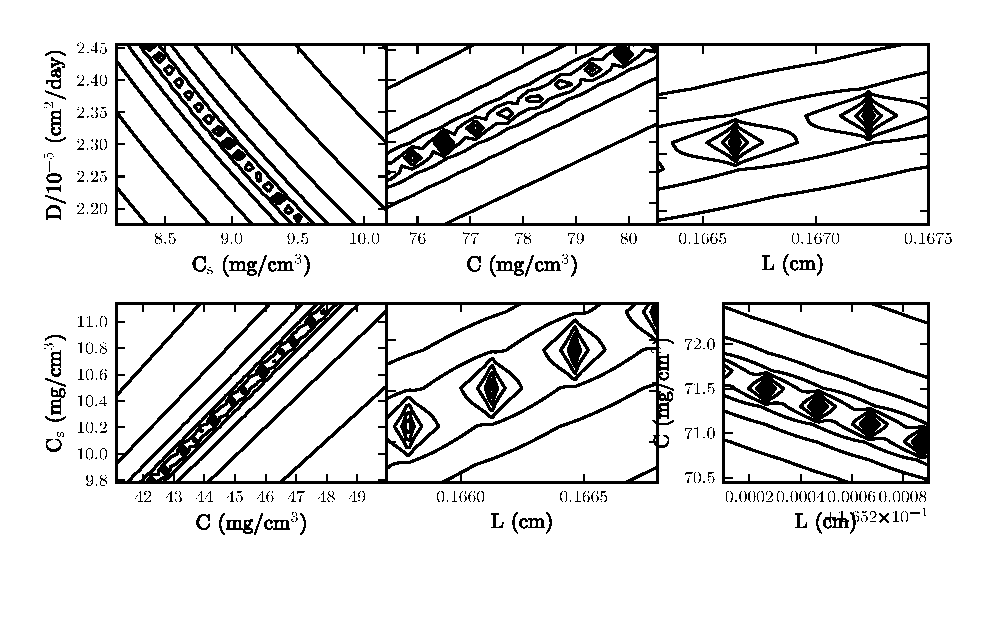
\includegraphics[width=0.75\textwidth]{figures/higuchi_proj_zoom.eps}
  \caption{These plots are the zoomed up square regions in black of the previous 
    Figure. One can see that the ridges consist of several
    local minima. Their number and depth will increase as the image is more finely 
    resolved.
  }
  \label{fig:higuchi_zoom}
\end{figure}
\clearpage
%=============================================================================
\begin{table}
  \caption{Parameters defining the reference profile and its envelop
    delimited by the upper and lower curves.
    These simulation parameters were used for the training of the neural network model
    proposed by ~\cite{Reis2004} and are also adopted as a benchmark of the present algorithm.
    Note that the size of the envelop actually encompasses the four different matrices 
    analyzed by ~\textcite{Fu1976} for the experimental release of hydrocortisone 
    ($\sim 3\% - \sim 60\%$ release after $100$ days).
  }
  \label{tab:ranges}
  \begin{ruledtabular}
    \begin{tabular}{lrrrr}
      Parameter & Reference & Lower bound & Upper bound & bits \\
      \noalign{\smallskip}
      \hline
      $\Co/$(mg cm$^{-3}$)             & 70.0 & 33.3 & 133.1 & 10 \\
      $\Cs/$(mg cm$^{-3}$)             & 16.2 &  2.7 &  40.0 & 10 \\
      D/($10^{-5}$ cm$^2$ day$^{-1}$)   & 1.35 & 0.042 & 4.82 & 14 \\
      L/cm                            & 0.167 & 0.164 & 0.170 & 6 \\
    \end{tabular}
  \end{ruledtabular}
\end{table}
\clearpage

\begingroup
\squeezetable
\begin{table}
  \caption{Representative drug release profiles found by the aGA that
    are equivalent to our reference profile $\Qref$. 
    The last column shows the deviation \ldots
  }
  \label{tab:results}
  \begin{ruledtabular}
    \begin{tabular}{ccccc}
      $\Co$ & $\Cs$ & $D$ & $L$ & $\epsilon$ \\
      \noalign{\smallskip}
      \hline
      70.0& 23.0& 0.992& 0.1659& 2.1e-07\\
      130.4& 15.9& 2.419& 0.1672& 6.2e-03\\
      108.5& 38.0& 0.953& 0.1667& 6.7e-03\\
      44.9& 23.9& 0.731& 0.1698& 1.2e-02\\
      108.9& 20.0& 1.714& 0.1699& 1.3e-02\\
      77.1& 33.2& 0.812& 0.1664& 1.4e-02\\
      50.1& 22.2& 0.820& 0.1690& 1.5e-02\\
      57.1& 36.6& 0.616& 0.1646& 1.7e-02\\
      119.2& 36.6& 1.026& 0.1641& 1.8e-02\\
      73.0& 6.7& 3.055& 0.1643& 2.0e-02\\
      46.5& 18.4& 0.876& 0.1675& 2.1e-02\\
      46.5& 18.4& 0.876& 0.1675& 2.1e-02\\
      68.7& 23.8& 0.940& 0.1649& 2.4e-02\\
      46.2& 4.9& 2.739& 0.1666& 2.6e-02\\
      42.8& 3.0& 4.016& 0.1650& 3.4e-02\\
      131.5& 33.9& 1.190& 0.1643& 3.4e-02\\
      70.7& 32.7& 0.796& 0.1691& 4.3e-02\\
      87.4& 39.8& 0.798& 0.1684& 4.9e-02\\
      73.1& 29.4& 0.888& 0.1698& 5.1e-02\\
      126.0& 36.7& 1.125& 0.1682& 5.4e-02\\
      97.6& 23.6& 1.331& 0.1691& 6.0e-02\\
      97.6& 23.6& 1.331& 0.1691& 6.0e-02\\
      78.8& 39.7& 0.713& 0.1646& 6.2e-02\\
      70.1& 16.2& 1.350& 0.1670& 6.2e-02\\
      80.8& 32.6& 0.888& 0.1698& 6.7e-02\\
      121.0& 31.7& 1.173& 0.1643& 6.8e-02\\
      96.8& 9.8& 2.787& 0.1643& 8.5e-02\\
      46.6& 4.9& 2.725& 0.1654& 8.5e-02\\
      33.8& 17.7& 0.722& 0.1680& 9.0e-02\\
      120.4& 7.3& 4.676& 0.1668& 1.3e-01\\
    \end{tabular}
  \end{ruledtabular}
\end{table}
\endgroup
\clearpage

%=============================================================================

\end{document}

% Suppose a fitness function is multimodal, i.e, several peaks a GA will tend
% to converge to one of the peaks, particularly if one of the peaks is more
% fit than the others. Perharps, one likes to identify the peaks convergence to 
% several peaks simultaneously. A  'niche' can be thought of as one of the
% peaks and a 'species' is a collection of population members well suited for a
% particular niche. We might want a GA to create stable subpopulations (species)
% that are well suited to the niches. 


% The random immigrant mechanism aims to increase the diversity
% of the population including new individuals into the existing generatation
% to act in response to changes occurred in the environment ando to avoid
% premature convergence.
 

% BGA is an efficient stochastic search technique in which a group of candidate solutions
% evolves, through Darwinian principle of natural evolution Holland (1975) and Goldberg
% (1989), to an optimal solution via the application of genetic operators

% In GA-based optimization, it is required to encode values
% as individual chromosomes. Binary, gray, and floating-point
% coding are the three methods commonly used [23].
% The binary representation has some drawbacks when applied
% to multidimensional, high-precision problems. For example, for
% 100 variables with domains in the range , where a
% precision of six digits after the decimal point is required, the
% length of the binary solution vector is 3000. This, in turn, generates
% a search space of about 10 . For such problems GAs
% perform poorly.
% In floating-point coding, each chromosome vector is coded
% as a vector of floating-point numbers of the same length as the
% solution vector. Each parameter is forced to be within a desired
% range and the operators are carefully designed to preserve this
% requirement. The motivation behind floating-point coding is to
% move the GA closer to the problem space.
% A gray coding representation has the property that any two
% points next to each other in the problem space differ only by one
% bit. In both binary and gray coding, precision is sacrificed with
% an increase in domain size for a given, fixed number of bits. A
% floating-point coded chromosome on the other hand is capable
% of representing quite large domains it is also much easier to
% design special tools for handling nontrivial constraints [23].




%% highly complex combinatorial problem

%% GA's are global stochastic optimization tecniques that are based on the adaptive mechanics of evolution via
%% natural selection.

% The genetic algorithm exploits the higher-payoff, or "target," regions of the solution space, because successive 
% generations of reproduction and crossover produce increasing numbers of strings in those regions. The algorithm 
% favors the fittest strings as parents, and so above-average strings (which fall in target regions) will have more
% offspring in the next generation.


% In many design synthesis problems (both natural
% and artificial), it is beneficial to identify distinct
% clusters (species) of solutions that perform well. 
% These neighborhoods should be dnamically determined , for example by a fuzzy clustering algorithm, in order to 
% promote speciation, and to give the oportunity for diverse alternatives to survive.
% Clustering, in general, is a process of grouping several objects into a set of clusters, each of which contains
% the objects that are similar to each other in some way. 
% In fuzzy clustering each object belongs gradually to each of the clusters.


%% PERFECT SINK

%% GA, invented by Holland in the early 1970s, as a stochastic global
%% search method that mimics 
%% the metaphor of natural biological evaluation. GAs operates on a population of candidate 
%% solutions encoded to finite bit string called chromosome. In order to obtain optimality, 
%% each chromosome exchanges information by using operators borrowed from natural genetic to 
%% produce the better solution. GAs differ from other optimization and search procedures in 
%% four ways[14]:

%% (1) GAs work with a coding of the parameter set, not the parameters themselves. 
%% Therefore GAs can easily handle the integer or discrete variables.

%% (2) GAs search from a population of points, not a single point. 
%% Therefore GAs can provide a globally optimal solution.

%% (3) GAs use only objective function information, not derivatives or other auxiliary knowledge. 
%% Therefore GAs can deal with the non-smooth, non-continuous and non-differentiable functions 
%% which are actually existed in a practical optimization problem.

%% (4) GAs use probabilistic transition rules, not deterministic rules.

%% In this section we describes the main features of Modified Co-Evolutionary Genetic Algorithm 
%% (M-COGA)[15]. The main idea behind this algorithm is based on the ideas of co-evolution and 
%% repair algorithms (repair unfeasible solution).

%% It combines concept of co-evolution, repairing procedure (Repairing unfeasible solution) 
%% and elitist strategy. Repairing procedure, repairs the unfeasible points to satisfy the 
%% feasible space Click to view the MathML source. Elitist strategy is used to produce a faster 
%% convergence of the algorithm to the optimal solution of the problem. 
%% The working procedure of M-COGA is described in the following manner:


%% Although neural networks were first suggested in the early 1940s, it
%% is only in the past 15 years or so that they have been used with some
%% success as systems that can learn to recognize patterns in a variety
%% of scientific and industrial applications. Conventionally they consist
%% of layers of cells (artificial neurons) where interconnections between
%% neurons in adjoining layers are made through 'weights', while the body
%% of the cell performs summations that cause it to 'fire' at an output
%% (the axon) when the incoming weigthed activity overcomes some
%% mathematically specified gradient function. The weights are thought to
%% resemble the action of synapses in real neuronal cells found in
%% biological brains, where neurons connect and learning takes place
%% through the alteration of such weights.So an artificial network (which
%% can have one of many popular topologies) learns to approximate an
%% input-output function by being given examples of the in- and
%% out-values of such a function. It does this through one of a variety
%% of weight-adjustment procedures known as learning algorithms. The
%% learned tasks can be as esoteric as recognizing faces where it would
%% be hard for a programmer to work out a priori a function that would
%% distinguish between such patterns. 

